% !TeX root = ../main.tex

\chapter{系统详细设计与实现}
本章将从具体的细节上着手阐述系统中各个功能模块与架构模块的具体实现,重点在于内部算法和数据结构的设计与实现。

\section{流水线管理}
流水线管理主要包含对流水线中各个子概念及其操作的封装,包括流水线实体类、流水线运行记录类、阶段实体类、阶段运行记录类、作业实体类、作业运行记录类、任务实体类、任务运行记录类。
类图如图\ref{fig:流水线管理类图}所示。
\begin{figure}[h]
  \centering
  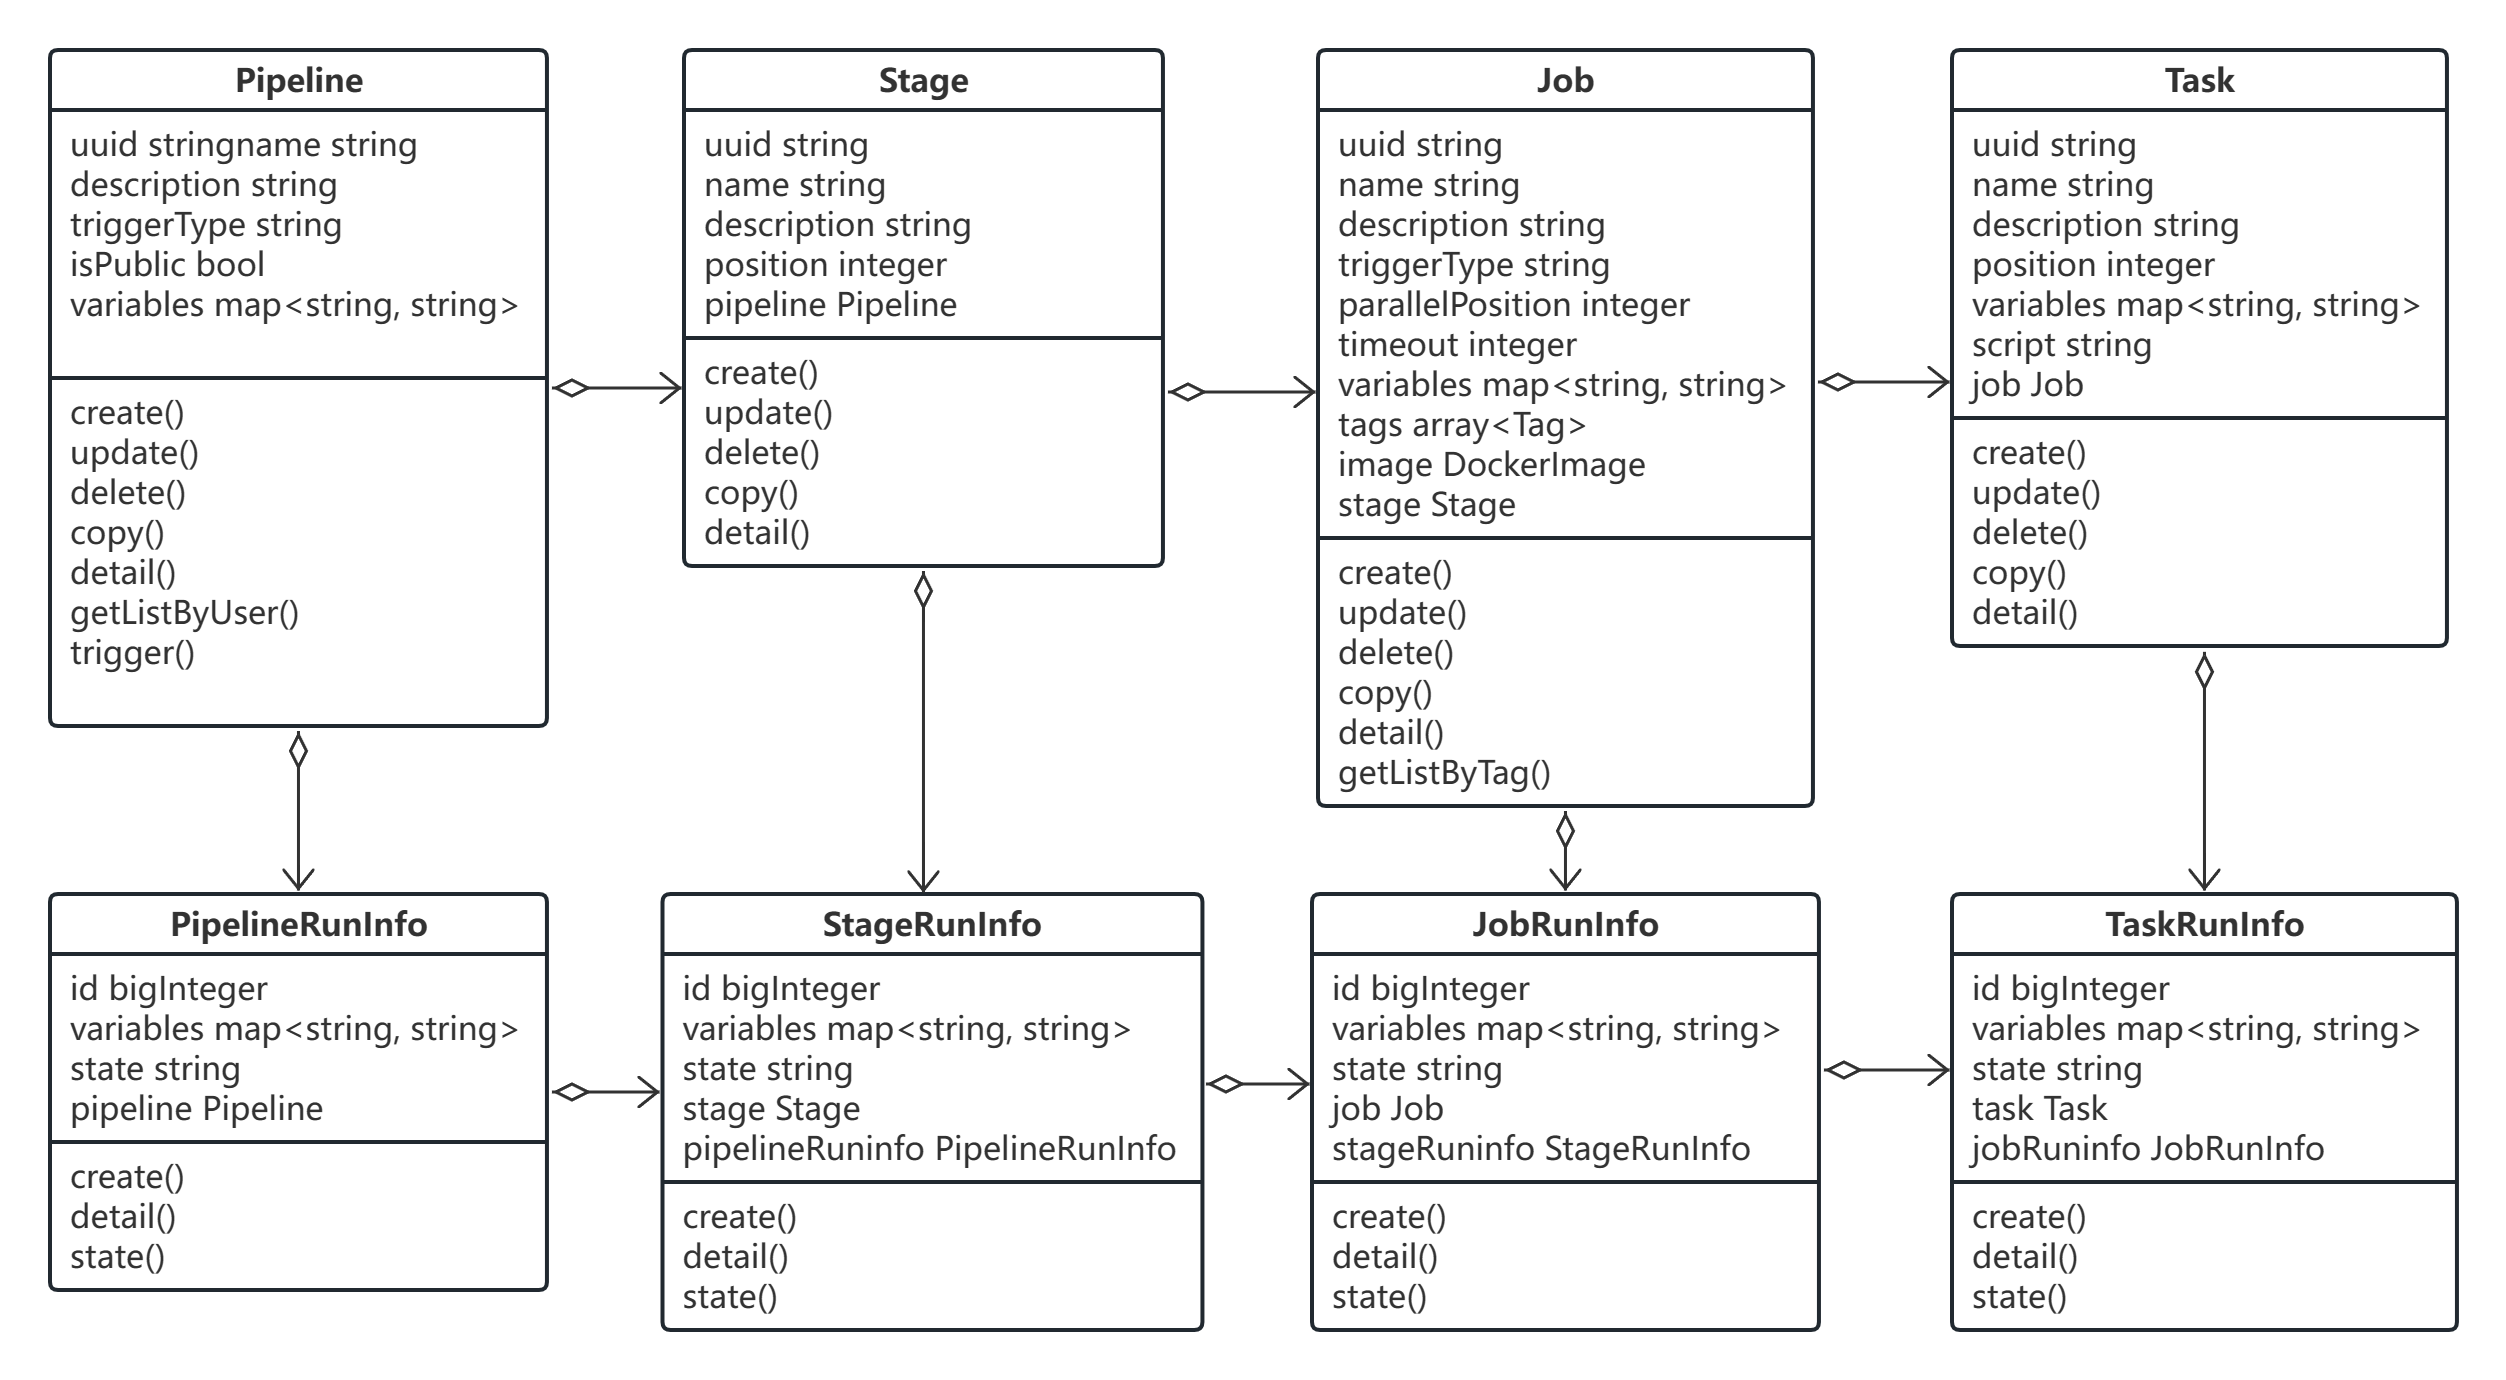
\includegraphics[width=1\textwidth]{流水线管理类图.png}
  \caption{流水线管理类图}
  \label{fig:流水线管理类图}
\end{figure}

\subsection{创建并配置流水线}

用户创建流水线时,系统会调用Pipeline.create()创建出一个空白的初始化流水线,同时其中会递归地调用一次Stage.create()方法创建其内部的一个阶段,
同理Job.create()和Task.create()也会被调用。在流水线管理的相关类中,Pipeline类的大部分成员方法都会递归地向下层调用其所属的子概念实体的对应方法,
以保证增删改查对于整个流水线均生效。当用户创建作业时,在填写基本信息的基础上,还需要在系统所管理的镜像库中指定一个镜像,该作业会在该镜像进行构建出的容器中执行,
如果用户没有合适的镜像选择,系统将会暂存当前用户所构建的流水线配置和结构,跳转到镜像管理界面来引导用户创建镜像。
同时,用户需要为作业指定合适的Tag标签,作业的运行环境可能需要在指定的服务器上运行,以满足其硬件环境要求,作业会通过消息队列被分配到Tag匹配的节点中运行。
每当用户保存当前已经创建并配置好的流水线时,系统都会实时调用Pipeline.detail()方法,以保证用户能够实时查看到当前的流水线配置。

\subsection{触发流水线}

对于流水线的触发,首先将从流水线实体开始调用Pipeline.trigger()方法,该方法中将递归地调用其包含的所有阶段实体的Stage.trigger()方法,
此后每个阶段实体会调用其包含的所有作业实体的Job.trigger()方法,同理调用任务实体的Job.trigger()方法。
每个实体的trigger()方法首先会根据自身的属性创建出对应的运行记录对象实体,并调用Pipeline.create()方法,与上述的trigger()方法类似,
这一方法会递归调用其下的PipelineRunInfo、JobRunInfo和TaskRunInfo的create()方法,创建出与流水线嵌套结构相同的运行记录实体,并存储到数据库。

创建运行记录实体的过程完成后,Backend模块将把当前流水线的结构与配置转化为Json格式发送给调度器。
此后由调度器中的作业中心进行接收并调用JobManager.addJob()进行进一步封装后,
交由调度器中的决策中心发出TriggerEvent触发事件,作业中心将调用JobManager.SubmitJob()将作业交付塞入消息队列中。
最后与作业Tag匹配的节点中的执行器将会从消息队列中得到该作业并开始执行。

\section{镜像管理}
镜像管理的实现主要涉及到对Docker镜像及其操作的封装抽象,以及对Layer层的管理。类图如图\ref{fig:镜像管理类图}所示。

\begin{figure}[h]
  \centering
  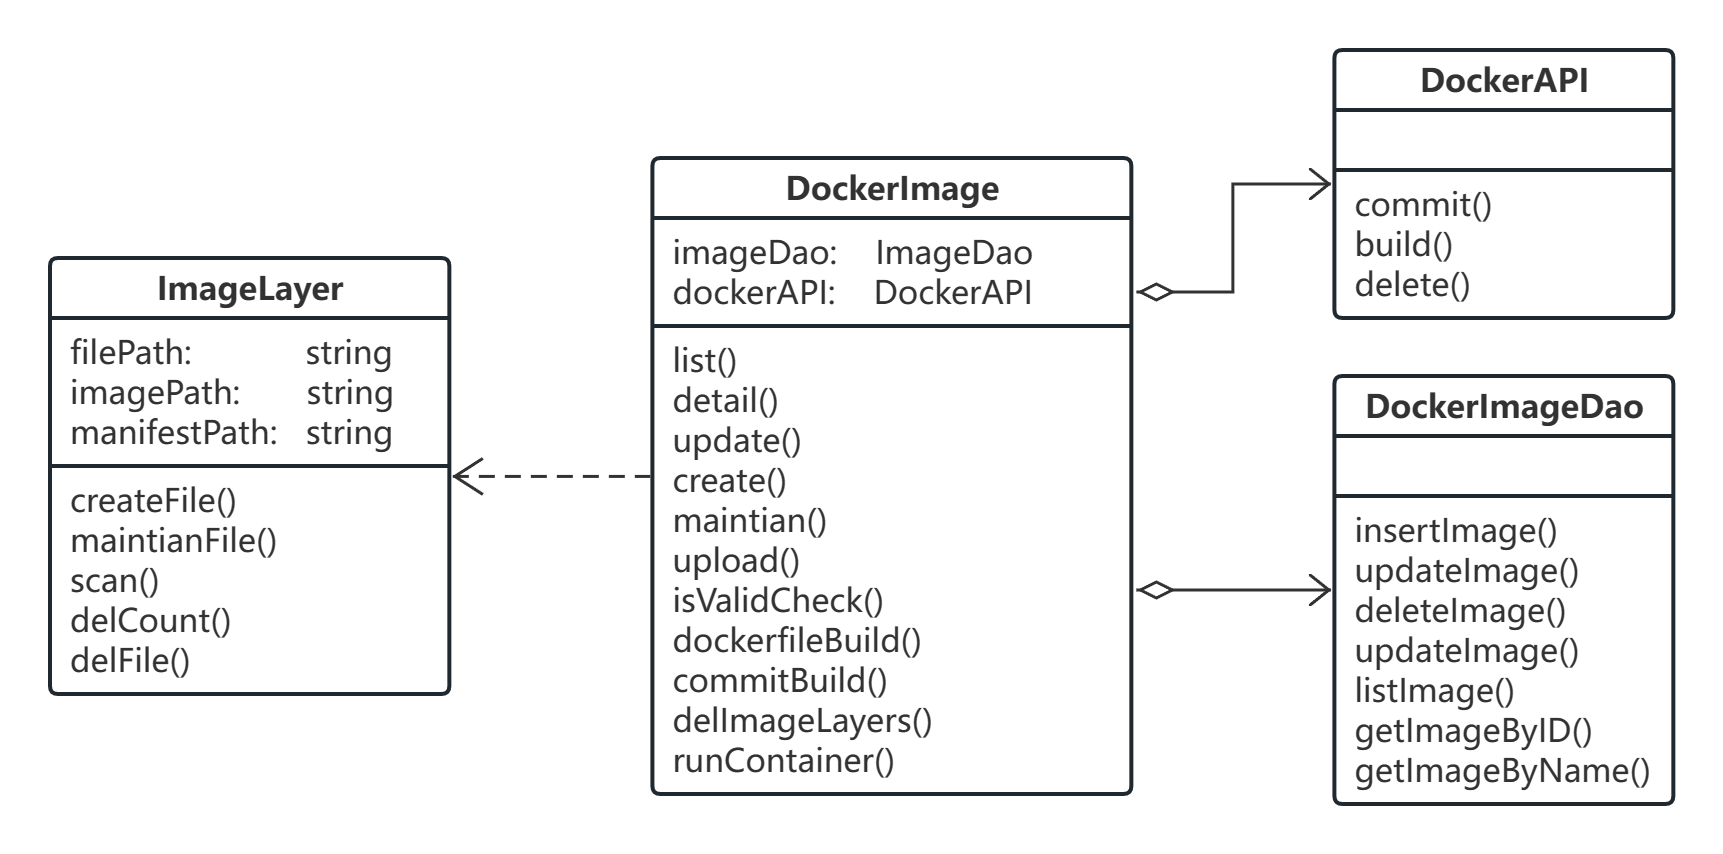
\includegraphics[width=1\textwidth]{镜像管理类图.png}
  \caption{镜像管理类图}
  \label{fig:镜像管理类图}
\end{figure}

\subsection{制作镜像}
制作镜像首先需要用户填写一系列基本信息,包括:镜像名称、镜像描述、镜像标签(Label)等,之后系统会实例化一个DockerImage类对象,
该类对象则包含了一些镜像的属性以及相应操作。

系统首先调用DockerImage.isValidCheck()来检测基础内容是否符合要求,如镜像名称是否有重复,镜像标签是否包含非法字符等。
然后,根据用户传入的制作选项,分别调用不同的制作策略:如果是Dockerfile的策略,系统将调用DockerImage.dockerfileBuild()方法并传入用户传入的文件,
方法内部将ssh进入系统的setting文件中配置的镜像制作服务器,执行docker build命令来直接构建镜像,最后将镜像传入镜像仓库;
如果是Commit策略则首先系统将调用DockerImage.commitBuild()方法,方法内部会在镜像服务器中根据用户配置的基础镜像,执行docker run来启动一个容器,并暴露出容器内部的ssh端口,
此后前端通过Wetty连接容器,此后用户便可以在用户界面使用终端进行操作。
注意,为了保证系统的安全性,我们需要对用户请求进行验证,如果不进行验证,当外部恶意模拟用户请求在服务器中创建容器,并通过一些手段影响到宿主机,会给系统带来极大的安全隐患。

\subsection{上传镜像}
根据在\nameref{subsec:镜像管理}中的分析,为了保证能够充分利用镜像仓库空间,确保不需要的镜像被完全删除,在镜像的上传和删除过程中均需要对Layer进行维护。
首先,前端发送上传镜像请求后,系统将调用DockerImage.upload()方法,该方法内部会判断DockerImage实例对象是否有label属性,根据label标签使用docker push命令推送至不同的仓库,如果没有标签则默认推送至公共仓库。

最后则需要进行Layer操作,首先实例化出ImageLayer实例,调用ImageLayer.scan()方法需要检测Layer文件是否存在,如果不存在则调用ImageLayer.createFile()方法,存在则调用ImageLayer.maintianFile()方法。

ImageLayer.createFile()和ImageLayer.maintianFile()方法会扫描Docker镜像的Manifest文件,将其中引用的ID与Layer实例的ID进行一一比较,从而判断Manifest文件中是否有引用该Layer,如果有则引用数加一,
如果没有则将Layer ID添加到引用文件中并设置引用值为1。这两个方法的区别在于ImageLayer.createFile()需要扫描所有的Manifest文件,而ImageLayer.maintianFile()只扫描指定的Manifest文件。

上传镜像时序图如图\ref{fig:上传镜像时序图}所示。

\begin{figure}[h]
  \centering
  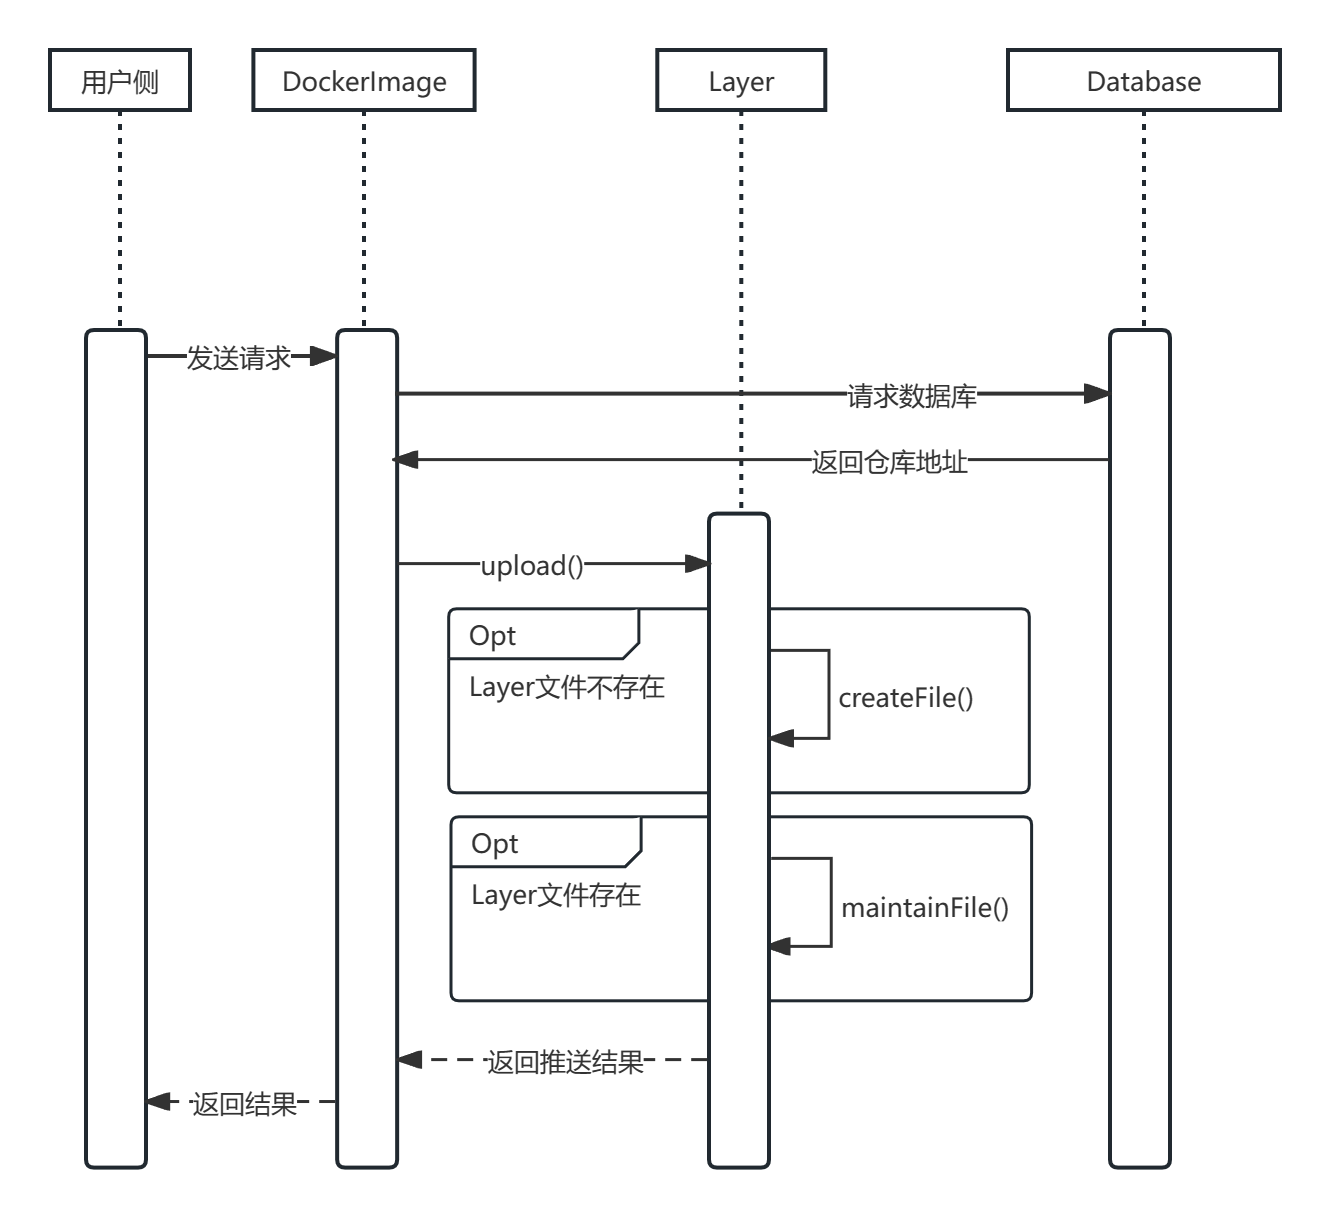
\includegraphics[width=1\textwidth]{上传镜像时序图.png}
  \caption{上传镜像时序图}
  \label{fig:上传镜像时序图}
\end{figure}

\subsection{删除镜像}
镜像由多个镜像层组成,并不是直接存储整个镜像本身,而是存储构成镜像的各个层。
对于每个Docker镜像,私有仓库利用一个Manifest配置文件来记录镜像所依赖的各层信息。当多个镜像共享同一层时,在仓库中该层只会被存储一次。
为解决以上问题,本模块优化了Docker官方的API,克服了无法移除底层文件的限制。这一过程主要包括两个阶段:首先扫描并移除不再需要的镜像层,然后利用Docker API删除相应的Manifest文件。

当需要删除特定镜像时,需对其引用的层进行移除。
我们通过DockerImage.delImageLayers()方法发起移除无效镜像层的请求。
鉴于可能有多个镜像引用同一层的情形,系统必须检查待删除的层是否还被其他镜像所引用。
直接检索每个镜像的Manifest文件以查找层引用会过于复杂,所以系统中为每个镜像层建立一个引用计数文件,记录层的ID和引用次数。
删除镜像时,相应层的引用计数减一。当某层的引用次数降至零时,系统将定位并直接删除该层对应的物理文件。
层的扫描、引用计数的减少及物理文件的删除分别由Layer.layerScan()、Layer.delCount()、Layer.delLayerFile()方法完成。

在移除引用计数文件和层文件之后,最后需调用Docker API来删除对应的Manifest文件,实现Manifest文件的最终删除。


\section{节点管理}
节点管理中对节点、标签和节点部署器中的属性与操作进行了封装抽象,其中节点部署器封装了一系列与节点服务器交互的方法,借助ShellHelper工具类完成使用shell语句与服务器间的交互。
类图如图\ref{fig:节点管理类图}所示。其中ShellHelper类是Shell语句的封装辅助类,将具体的shell语句与业务代码解耦。
Deployer则封装了节点管理中一切与节点服务器交互的方法,将服务器操作与Pod操作类解耦。
Pod类则表示了一个节点对象,与数据库中的一个一条节点记录一一对应,封装了一系列节点属性与节点操作。

接下来重点介绍节点的部署的详细设计。

\begin{figure}[h]
  \centering
  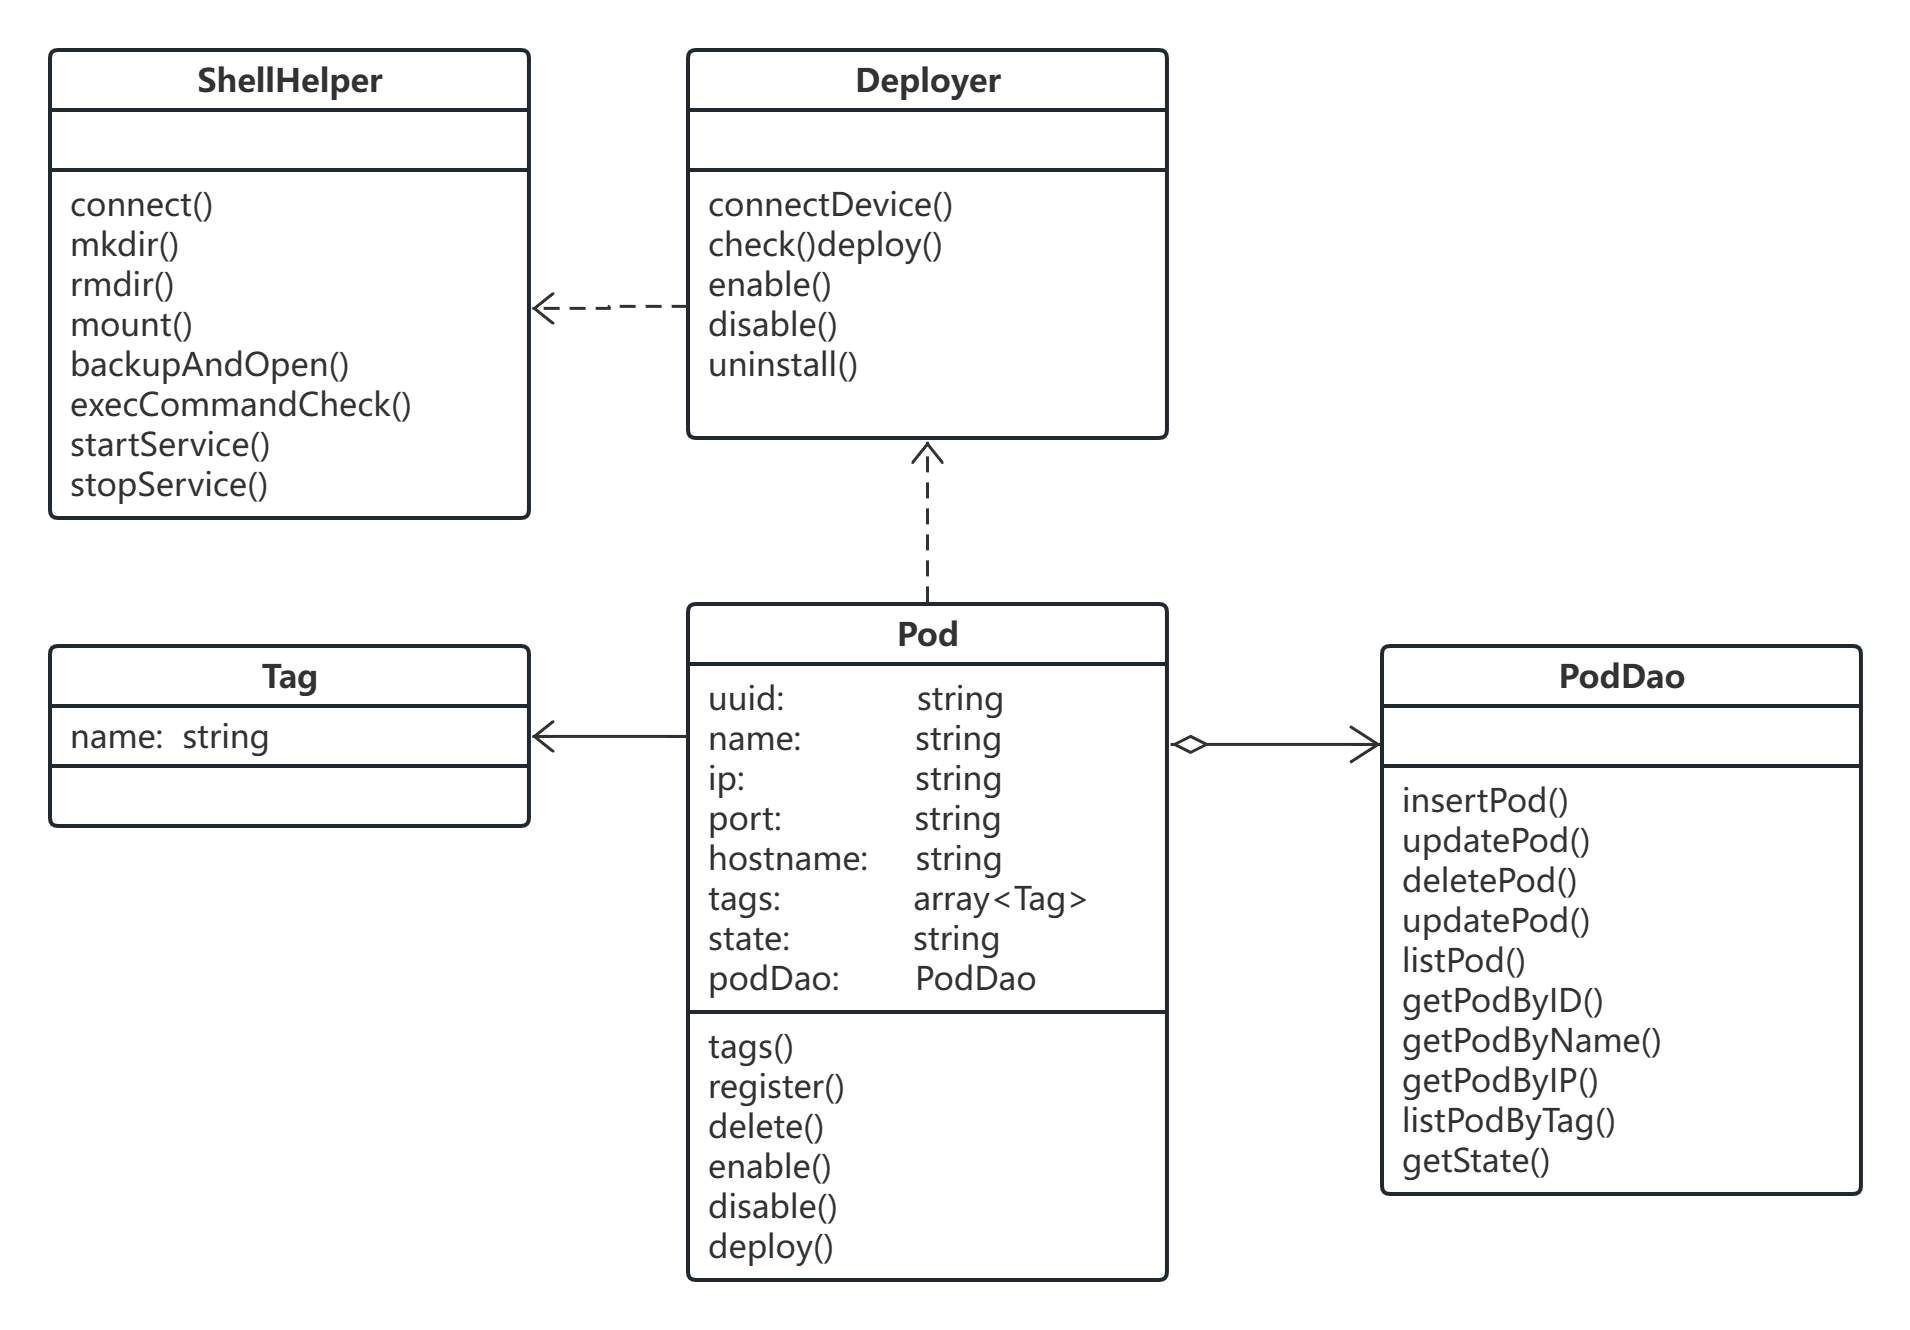
\includegraphics[width=1\textwidth]{节点管理类图.png}
  \caption{节点管理类图}
  \label{fig:节点管理类图}
\end{figure}

\subsection{节点一键部署}
首先,系统在ShellHelper类中设计了execCommandCheck()私有方法,这一方法包含了执行shell语句和检查shell语句两个功能,
如果shell语句执行过程中报错,会根据不同的错误类型返回不同的错误码,这一私有方法在其他方法中被大量调用。
其余ShellHelper类中的方法则是对递归创建文件、启动服务、停止服务等语句的封装,以供Deployer调用。

在节点部署的核心过程如下:首先需要调用ShellHelper.connectDevice()连接到目标服务器,然后递归创建预设的一系列目录结构,并备份原配置文件为bak文件,
分别由ShellHelper中mkdir()和backupAndOpen()方法实现。此后根据执行器的预设yaml文件对服务器配置文件进行写入,同时使用curl命令从远程拉取执行器的二进制执行文件。
此后便可以通过调用ShellHelper.startService()方法,该方法中包含三个部分:首先执行systemctl daemon-reload命令来重新加载配置文件,以保证执行器的配置是最新的,
然后执行systemctl enable来启动执行器服务,最后,自动化部署脚本中,还要执行systemctl restart以便确保所有配置的更改都被采用,并且服务是按照最新配置运行的。

\section{调度器的实现}

\subsection{状态转移模块的实现}

调度器中以状态机的设计模型来控制流水线中作业和任务的状态流转。
以下介绍作业状态机的详细设计,任务状态机与作业状态机极为相似,此处不再赘述。

按照有限状态机的设计理念,我们首先需要确定作业状态机的状态(State)和事件(Event)。
依据需求分析,系统中设计了以下作业状态:就绪中(Pending)、执行中(Running)、执行成功(Success)、执行失败(Failed)、被跳过(Skipped)和被取消(Canceled)。
同时设计了以下事件:触发(triggerEvent)、重试(retryEvent)、作业成功(successEvent)、作业失败(failEvent)、作业执行超时(timeoutEvent)、跳过(skipEvent)、取消(cancelEvent)、审核通过(reviewApproveEvent)和审核失败(reviewRejectEvent)。
依据状态机的设计模式,系统中将流水线作业的不同状态封装为类,将引起其状态转移的事件设置为成员方法。图~\ref{fig:作业状态机类图}为作业状态机类图。

\begin{figure}[h]
  \centering
  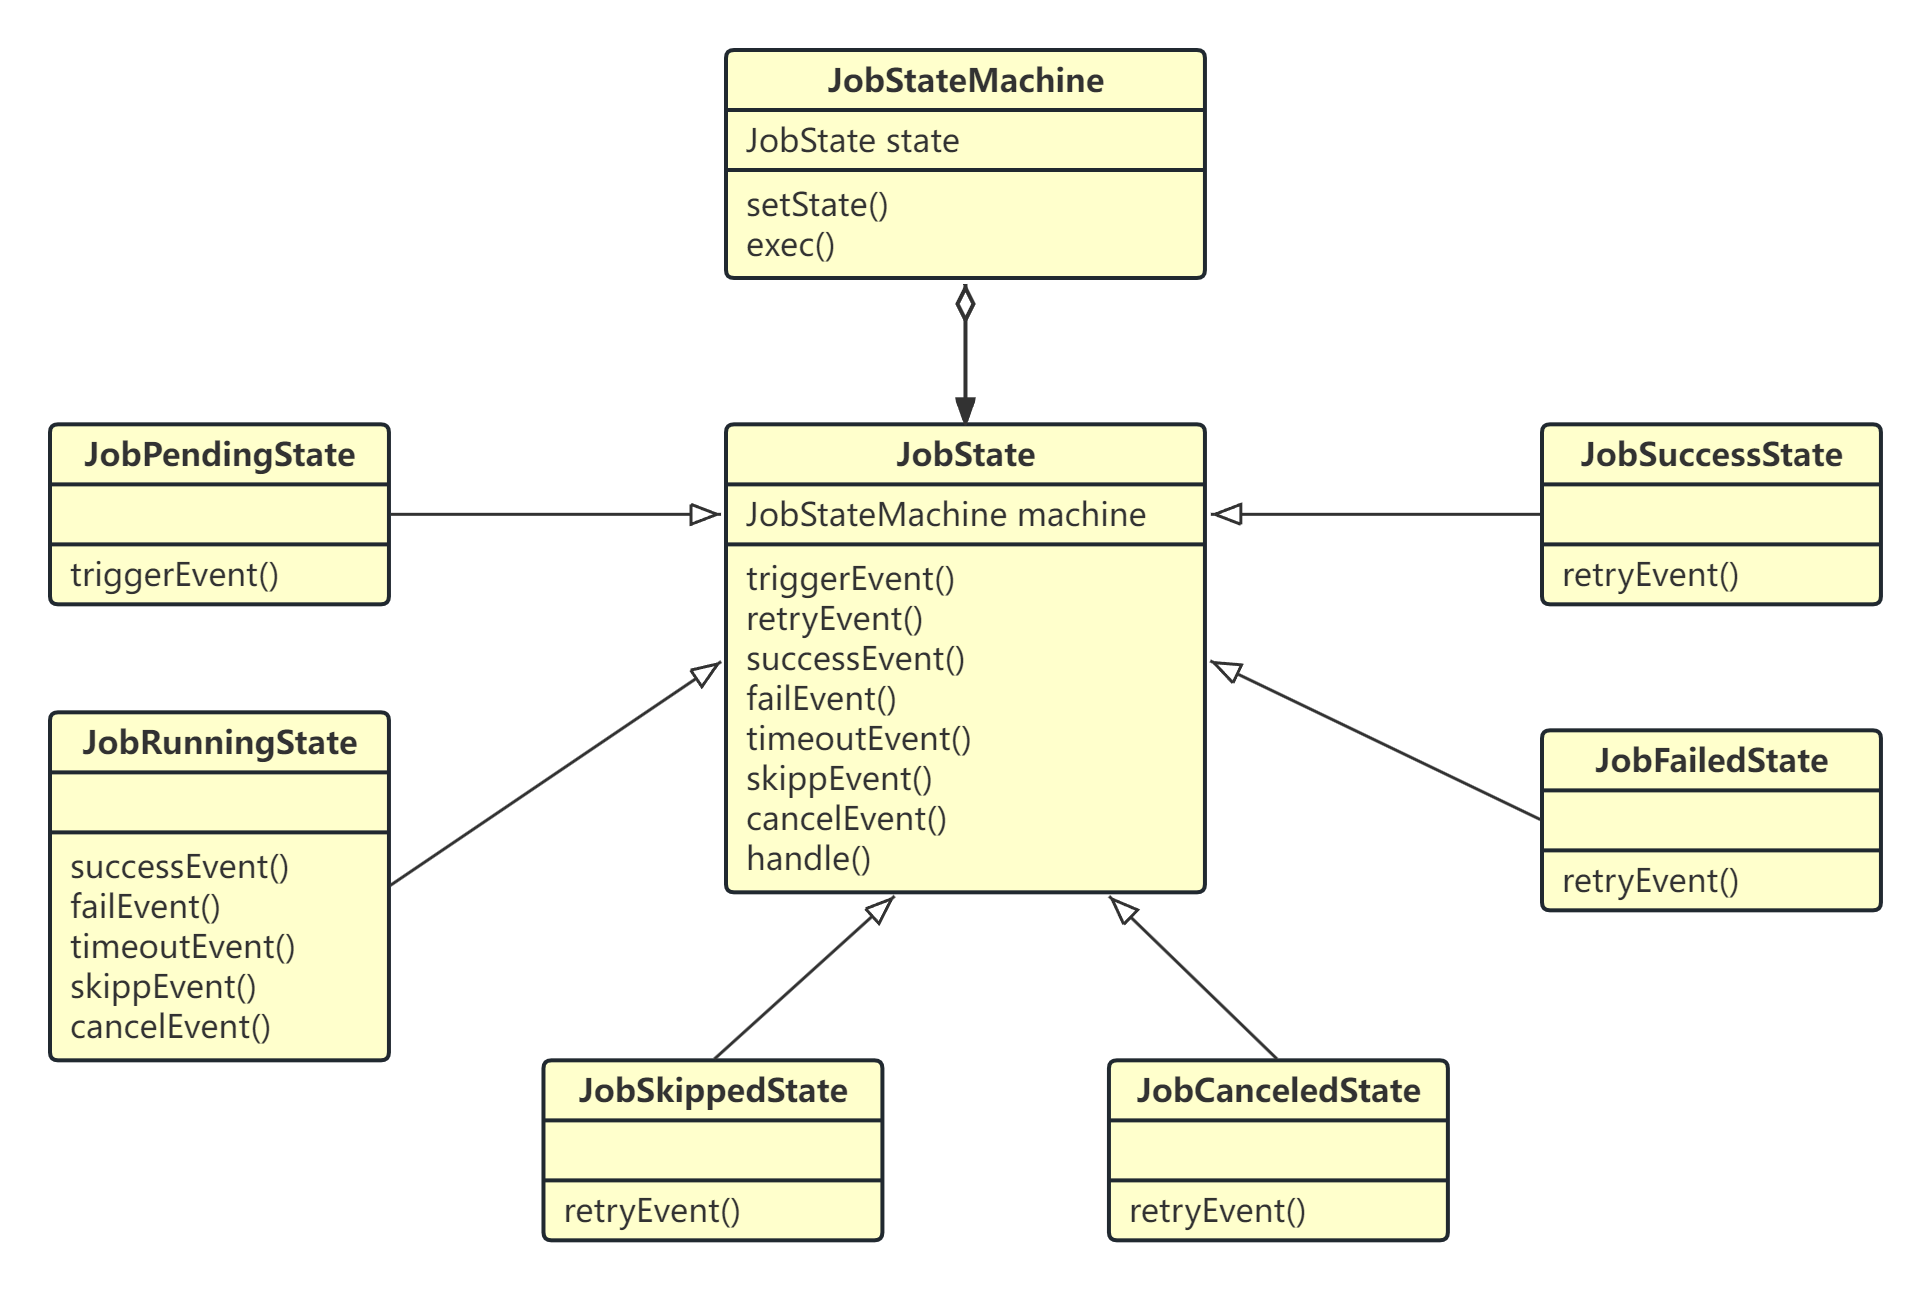
\includegraphics[width=1\textwidth]{作业状态机类图.png}
  \caption{作业状态机类图}
  \label{fig:作业状态机类图}
\end{figure}

当需要进行作业状态转换时,首先创建JobStateMachine实例并设置默认初始状态,然后向exec成员方法中传入当前发生的事件。
其中JobState是作业状态的抽象类,作业中每个具体的状态作为一个JobState的实现类,并从JobState中选择引起其状态转移的事件方法来实现。
例如JobRunningState类实现了JobState中的successEvent、failEvent、timeoutEvent、skippEvent和cancelEvent五个成员方法,这是因为这些事件均能作用于一个正在运行中的作业并且引起其状态改变,
其中successEvent方法会调用父类中持有的实例的JobStateMachine成员的setState方法,将当前状态机的状态设置为成功,并完成一些后续工作,其余事件方法也与之类似。

接下来具体分析作业状态机内部的状态转换:
当一个作业运行实例被创建时其应为就绪中状态,故就绪中(Pending)状态为初始状态,引发其状态改变的事件是触发(triggerEvent),这个触发事件是由决策中心经过决策逻辑发出的,并不只是用户的动触发行为,
一旦作业被成功触发,其状态则改变为运行中(Running);如果该作业被设定为需要人工审核才能触发,则审核通过事件(reviewApproveEvent)将会将状态改变为运行中(Running),审核驳回事件(reviewRejectEvent)将会将状态改变为失败(Failed)。
当作业处于运行中时,调度器可能会收到来自两方面的信号,其一是执行器所通知的作业执行状态,包括作业执行成功(successEvent)、执行失败(failEvent)和执行超时(timeoutEvent),
其中执行成功会使得作业状态机变为执行成功状态(Success),执行失败和执行超时都会变为执行失败状态(Failed);
其二是CI-Service所通知的用户人工干预命令,包括取消作业(cancelEvent)和跳过(skipEvent)作业,这两种事件会立即使得作业状态机变为取消(Canceled)和跳过(Skipped)状态。
以上两种信号均由决策中心先收到信号并统一处理决策后再转发给状态机,这样做可以统一外界信号的入口,降低其他模块与调度器间的耦合。
当处于运行中的作业进入终态后,作业仍然可以通过重试事件(retryEvent)来重新进入运行中的状态。
至于当前的作业是否满足触发该事件的条件,或者是否需要人工审核,由决策中心统一处理后发出信号,状态机不做额外的业务逻辑判断。

图~\ref{fig:流水线作业状态图}展示了作业状态机的状态流转。

\begin{figure}[h]
  \centering
  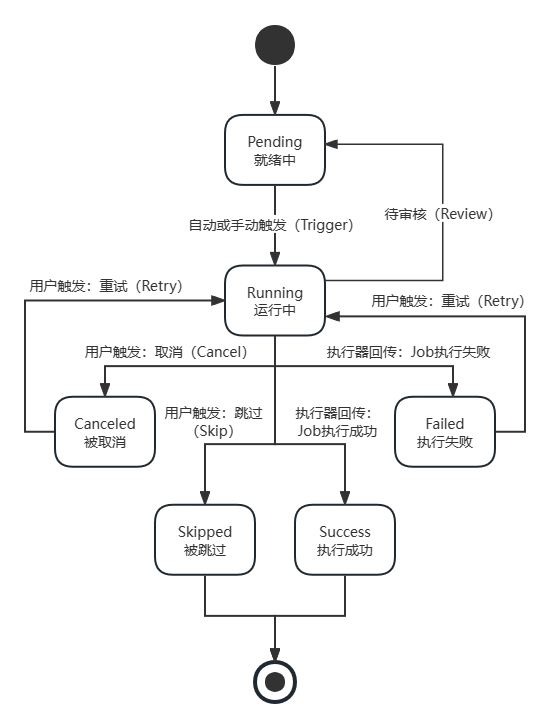
\includegraphics[width=0.7\textwidth]{流水线作业状态图.png}
  \caption{流水线作业状态图}
  \label{fig:流水线作业状态图}
\end{figure}

% 对于流水线和阶段的状态转移则相对比较简单。
% 对于阶段来讲,阶段的状态并不受到的具体的作业运行情况的影响,而是根据当前该阶段内所有作业的状态来综合决定,阶段状态机的类图如图\ref{}所示。

% 首先我们需要定义一套

\subsection{作业管理与决策中心模块的实现}

作业管理是调度器对Backend模块传入的作业信息进行二次封装和操作的模块。
决策中心则是整个调度器的核心模块,负责根据当前发生的事件(Event)和当前作业状态对作业管理模块中获得的作业进行决策。
作业管理与决策中心的类图如图\ref{fig:作业管理与决策中心类图}所示。

\begin{figure}[h]
  \centering
  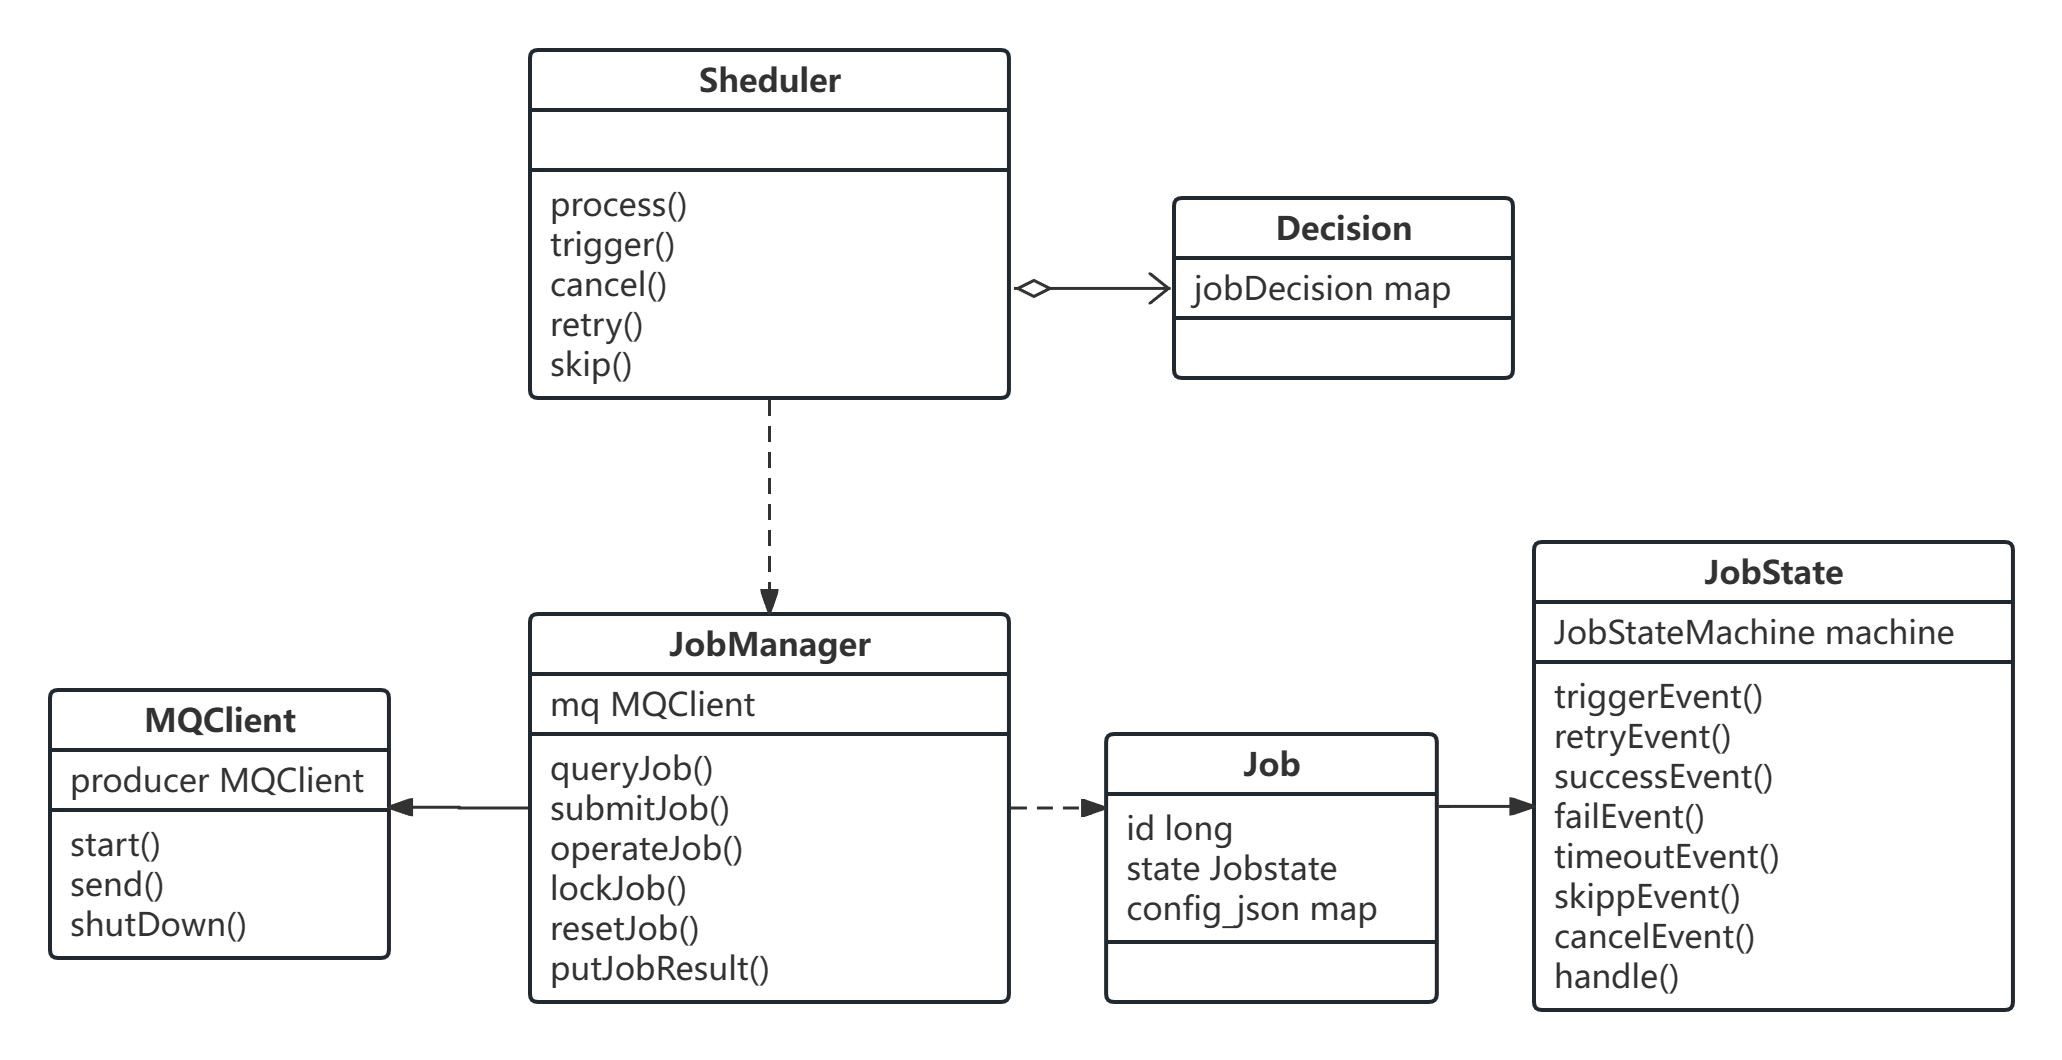
\includegraphics[width=1\textwidth]{作业管理与决策中心类图.png}
  \caption{作业管理与决策中心类图图}
  \label{fig:作业管理与决策中心类图}
\end{figure}

在整个调度器的核心代码中,Scheduler 类位于调度模块的核心位置,其主要负责执行一个关键功能:processTask()。该方法的主要职责是从作业管理器中拉取待处理的作业,并基于作业事件及其当前状态来做出相应的调度决策。
makeRunDecision()方法体现了该决策逻辑,而当决策包含特定的作业处理时,batchPutJobDecision则被用于执行相关操作。决策对象由Decision类封装,其中作业的决策以Map形式存在,以便支持作业的并行处理能力。
这其中会用到一个DecisionEnum枚举类,其中包含可能的决策事件并与作业状态机中的Event一一对应,这些事件直接影响流水线作业的执行和作业状态的转换。

作业管理(JobManager)和Scheduler交互是通过作业实体Job进行的,putJobResult()方法接受执行器返回的状态更新,并将相关作业重新排队等待下一轮调度决策。getUnackJobs()方法能够查询那些已经分发给执行器但尚未执行的作业。

系统初始化时,Scheduler.process()方法将在守护线程中运行,不断地处理作业。当Backend服务接收到用户发起的流水线事件时,会通过addJob()方法将作业提交至消息队列中进行排队。
此处需要注意,由于系统中调度器是多实例部署,属于分布式系统,任何一个节点都有可能处理这些作业,如此便产生了竞态条件,为了避免发生无法预期的错误,
以及保证作业不丢失,在进行决策前,必须通过JobManager.lockJob()方法对作业加锁,以获得处理权。

Scheduler在接收到一批待处理作业后,会根据每个作业的具体事件类型及其包含的状态进行详细决策。
完成决策后,决策结果Decision将被检查,如果包含对作业的决策,则将其发送回作业管理器以便进一步处理,这可能会导致作业状态的变更,则交由JobStateMachine进行处理。
若决策中未包含对整个作业的处理,而是针对特定作业的,则会触发作业管理器的相关处理逻辑,并通过后端服务进行状态持久化。
最后调用JobManager.releaseJob()对锁进行释放。

结合以上内容,作业调度时序图如图\ref{fig:作业调度时序图}所示。

\begin{figure}[h]
  \centering
  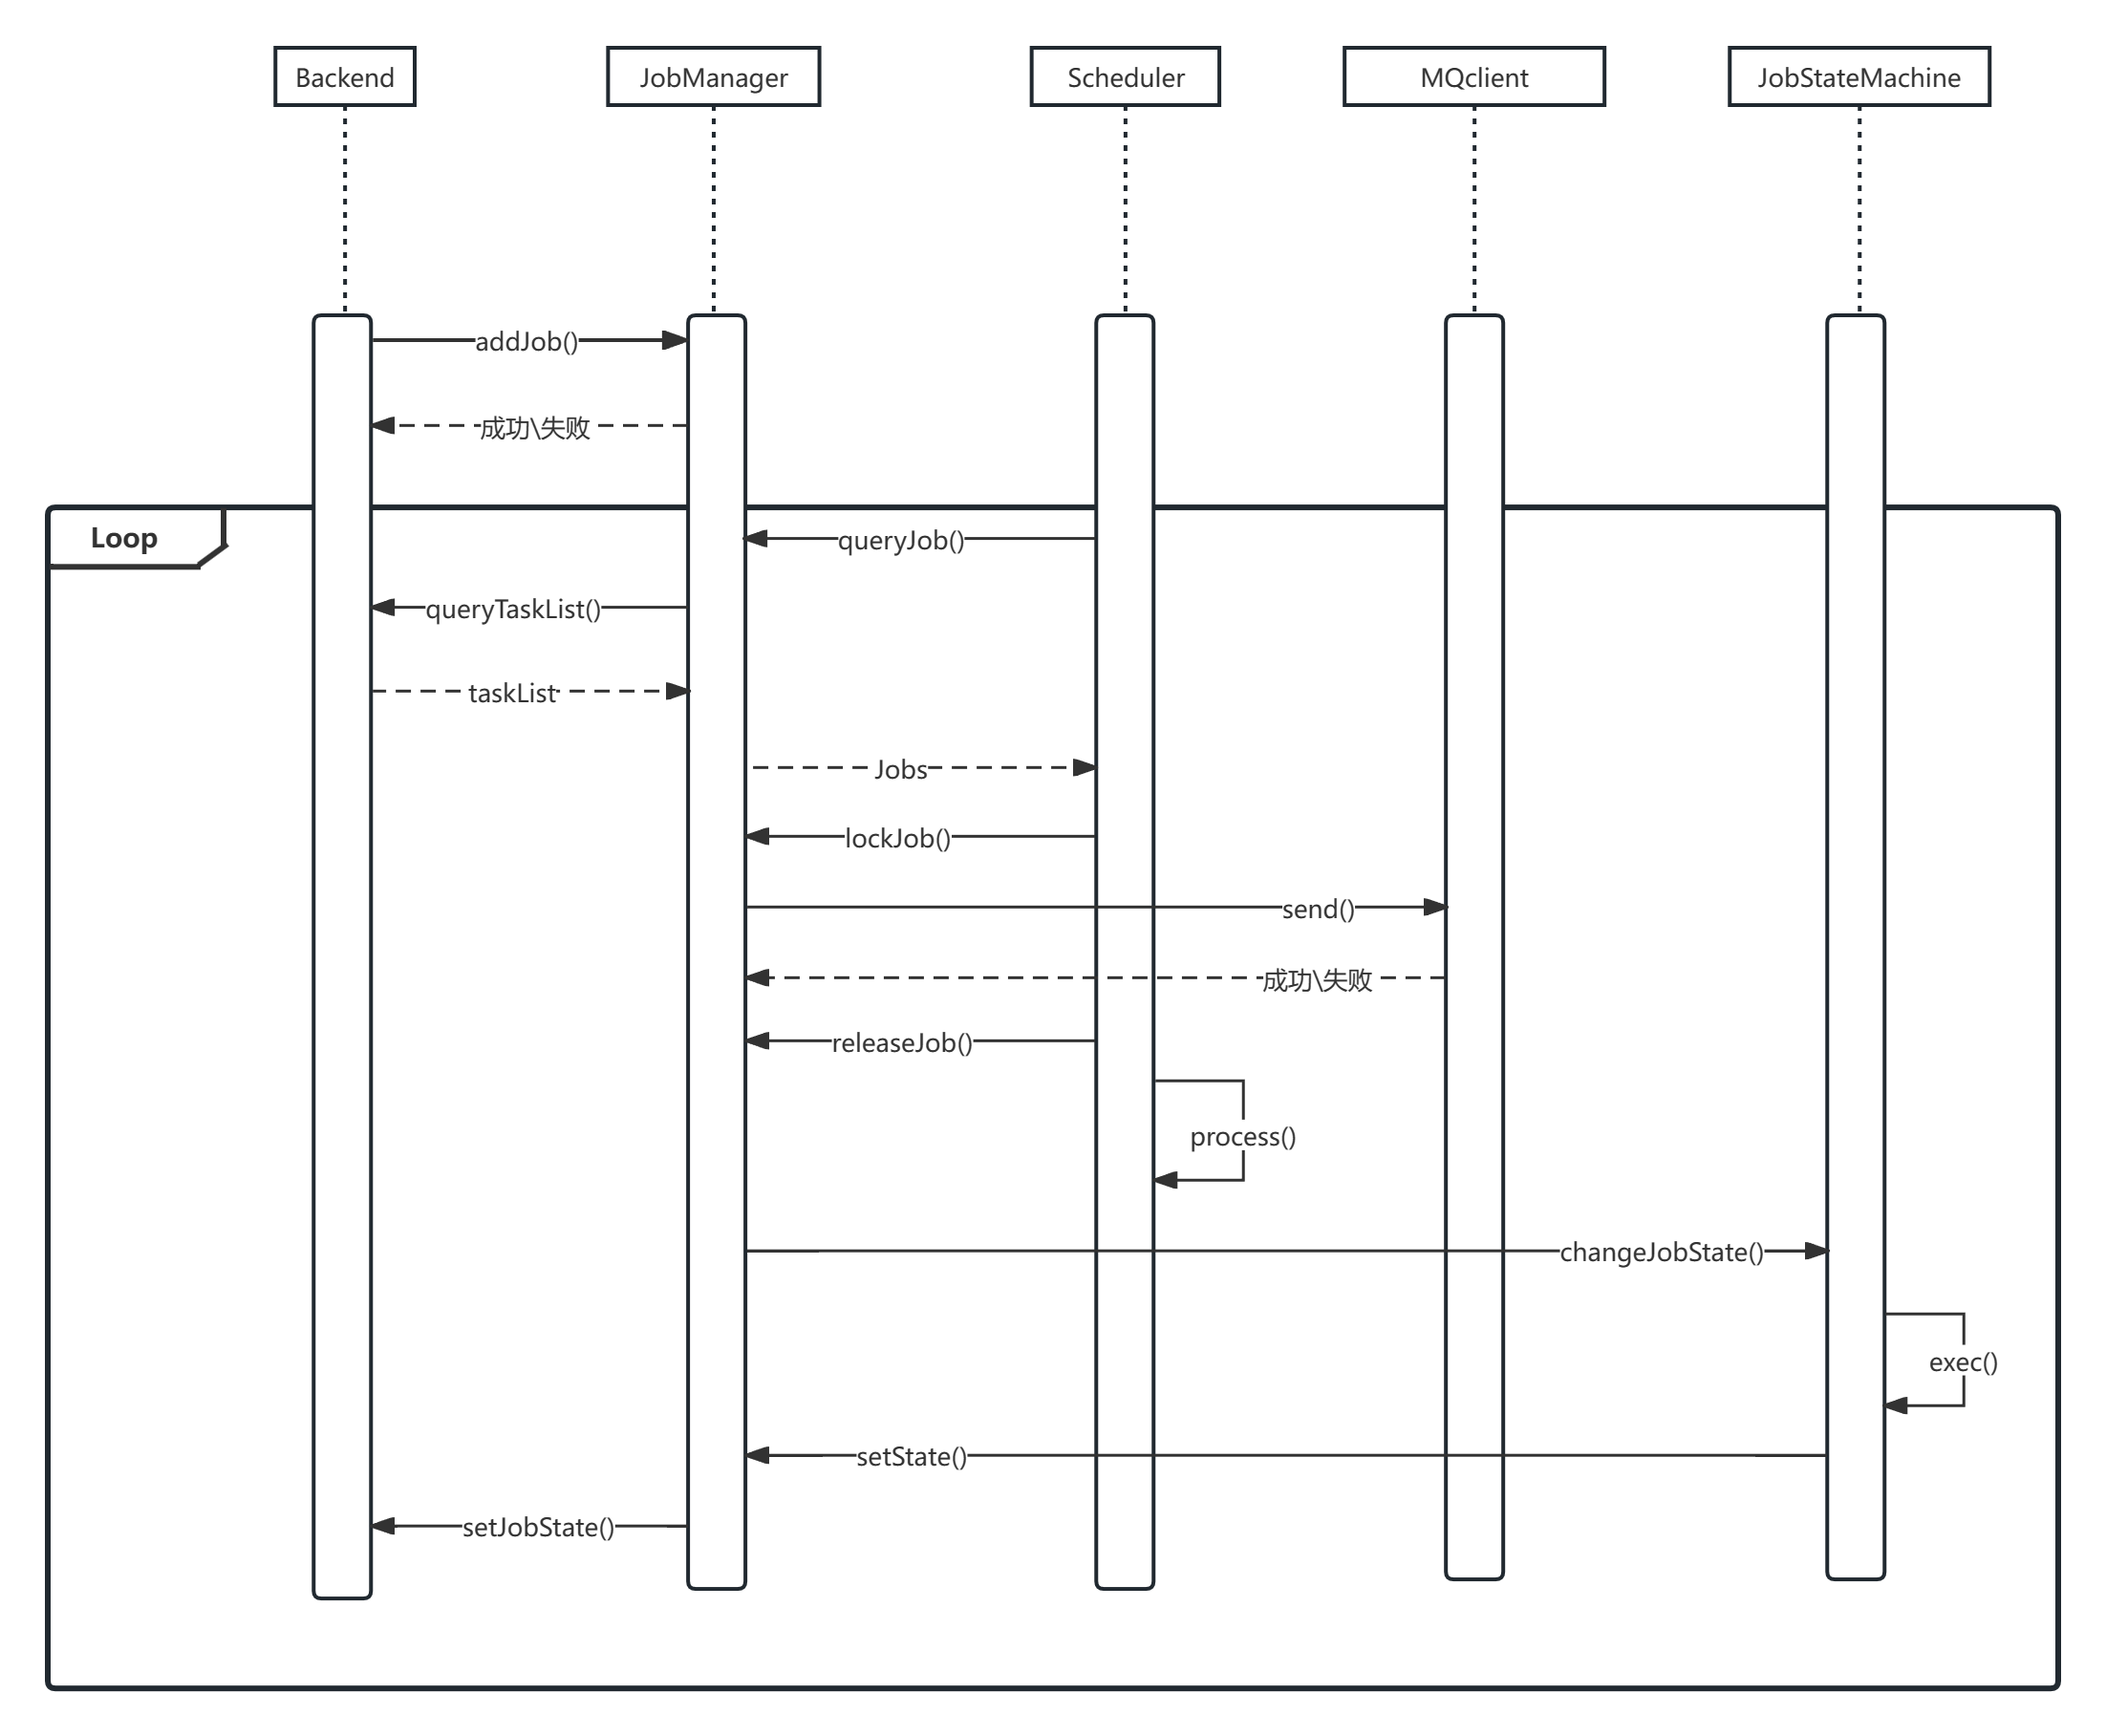
\includegraphics[width=0.8\textwidth]{作业调度时序图.png}
  \caption{作业调度时序图}
  \label{fig:作业调度时序图}
\end{figure}

\section{本章小结}
在本章中,我们深入探讨了容器化CI/CD流水线调度系统的详细设计与实现,重点关注了系统内部的算法、数据结构及其相互作用。
首先,流水线管理部分通过详细的类图和实例方法展示了如何高效地处理流水线的创建、配置与触发。特别是通过递归调用的设计,实现了从流水线到阶段、作业、任务的层层下达与信息同步,保证了流水线配置的一致性和执行的准确性。
镜像管理部分详述了如何在系统中创建、上传和删除Docker镜像。通过引入Layer层的概念,系统不仅简化了镜像管理过程,还优化了存储使用,提高了系统的整体效率和镜像的处理速度。
节点管理部分着重介绍了节点的一键部署功能,包括与节点服务器的交互、执行器的安装和配置,以及节点的上线与下线处理。此外,还强调了通过ShellHelper辅助类实现与服务器交互的灵活性和安全性。
调度器的实现部分则集中于系统的核心逻辑,即如何根据作业的状态和事件来做出合理的调度决策。通过有限状态机的设计模型,系统能够精确控制作业和任务的状态转换,同时确保作业的有序执行和资源的合理分配。
整体而言,本章从算法到数据结构,从功能设计到实现细节,为系统的构建提供了全面而深入的技术支撑,确保了系统的高效、稳定和可扩展。